\section{Einführung in die Programmierung}

\begin{frame}{Vorstellung}
\begin{itemize}
	\item Name
	\item Studiengang 
	\item Programmiererfahrung allgemein
	\item Programmiererfahrung Python
	\item Erwartungen
\end{itemize}
\end{frame}

\begin{frame}{Organisatorisches}
    \begin{itemize}
        \item Anwesenheitspflicht
        \item Teilnahmebestätigung (Zertifikat)
        \item "Regeln"
        \item Codio
        \item Skript
    \end{itemize}
\end{frame}


\begin{frame}{Die Programmiersprache Python}
\begin{columns}
    \column{0.5\textwidth}
    \begin{itemize}
        \item Warum Python?
            \begin{itemize}
                \item Flache Lernkurve, sehenswerte Ergebnisse bereits nach dem ersten Tag
                \item Verankert in Forschung und Wirtschaft
                \item Der englischen Sprache sehr ähnlich
            \end{itemize}
    \end{itemize}
    \column{0.5\textwidth}
    \centering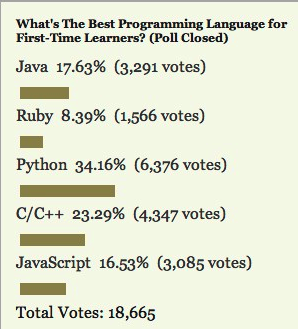
\includegraphics[scale=0.5]{images/best_lang} 
    \hyperlink{https://lifehacker.com/five-best-programming-languages-for-first-time-learners-1494256243}{\tiny{Quelle: lifehacker.com}}
\end{columns}
\end{frame}

